\section{Blade}
\label{sec:blade}

\begin{figure}[H]
    \centering
    
\includegraphics[scale=0.4]{images/blade.png}
    \caption{Logotipo da framework Blade.}
    \label{fig:blade}
\end{figure}

\hspace{5mm} A \textbf{Blade} consiste numa framework web (JavaWeb) simples/eficiente, onde as suas principais características no desenvolvimento são a performance e flexibilidade. 

\hspace{5mm} Do mesmo modo, esta framework também se caracteriza pela sua simplicidade, pois segundo os desenvolvedores da mesma, os utilizadores compreendem a \textbf{Blade} num único dia. A simplicidade deve-se ao facto de a framework não introduzir vários níveis entre o utilizador e as bibliotecas \textit{standard}.

\hspace{5mm} A framework \textbf{Blade} segue a arquitetura MVC (Model-View-Controller)

\hspace{5mm} As figuras seguintes (\ref{fig:blade-1},\ref{fig:blade-2},\ref{fig:blade-3} e \ref{fig:blade-4}), representam um \textit{Quick Start}, que pode ser consultado na página do GitHub da framework \textcolor{blue}{\textbf{\href{https://github.com/lets-blade/blade}{Blade}}}. Neste \textit{Quick Start}, abordam-se as capacidades da framework para a criação de aplicações web, monitorização do servidor e output (\textit{view}) dessa mesma aplicação.

\begin{figure}[H]
    \centering
    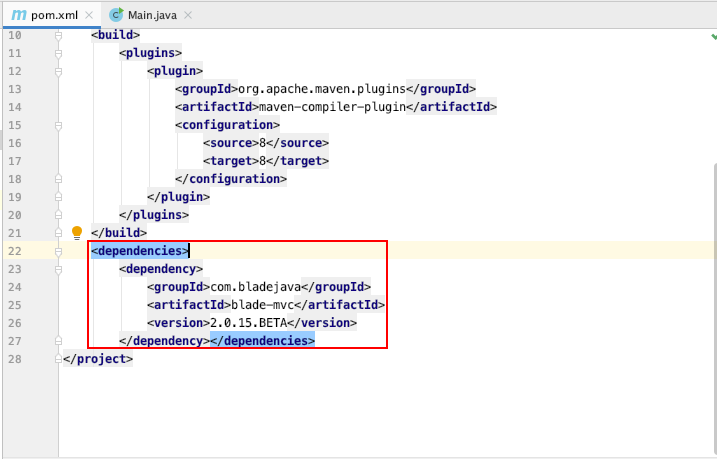
\includegraphics[scale=0.5]{images/blade-1.png}
    \caption{Ficheiro Maven com as dependências necessárias para utilização da framework \textbf{Blade} para este \textit{Quick Start}.}
    \label{fig:blade-1}
\end{figure}

\begin{figure}[H]
    \centering
    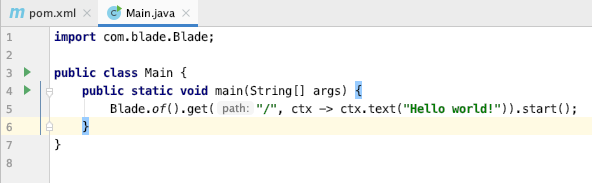
\includegraphics[scale=0.6]{images/blade-2.png}
    \caption{Código Java para \textit{Quick Start}.}
    \label{fig:blade-2}
\end{figure}

\begin{figure}[H]
    \centering
    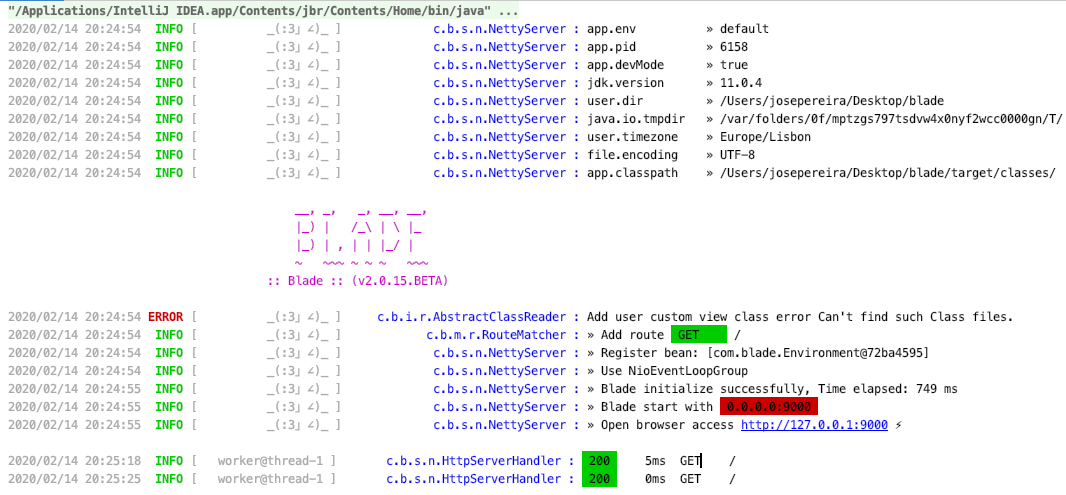
\includegraphics[scale=0.4]{images/blade-3.png}
    \caption{Monitorização do servidor web, fornecida pela framework \textbf{Blade}, onde se pode ver os pedidos.}
    \label{fig:blade-3}
\end{figure}

\begin{figure}[H]
    \centering
    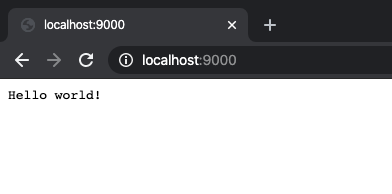
\includegraphics[scale=0.6]{images/blade-4.png}
    \caption{A aplicação web criada pela framework.}
    \label{fig:blade-4}
\end{figure}